%\documentclass{sig-alternate}
\documentclass[11pt,twocolumn]{article}
\usepackage{url}
\usepackage{graphicx}
\usepackage{subfig}

%\newcommand{\IGNORE}[1]{}

\title{Summer Research report}

%\numberofauthors{7}
\author{
  Lewis Barnett\\
  lbarnett@richmond.edu
}
\date{July 22, 2016}

\begin{document}

\maketitle
\begin{abstract}
  A brief (one paragraph) description of the work you did.
\end{abstract}


\section{Introduction}

This section should be a general description of the basic problem you
were trying to solve. 


\section{Related Work}

In this section, you would descripbe other similar work that has been
done by other researchers. For example: 
In \cite{BIRDID:Berg2013}, Berg and Belhumeur construct an image recognition
system with the goal of explaining to birders the differences between
similar species.

\section{Methods}
\label{sec:methods}

This section describes the methods used in your study. I am suppling
a subsection that you can use describing how the images were collected,
which you can use if you like. The rest of the section would be a
high level description of convolutional neural networks, the software
that you used, and any general setup information that needs
describing.

\paragraph{Image collection}

Images were collected using two motion-activated wildlife cameras, a Wingscapes BirdCam 2.0 and (when the original failed) a Wingscapes Birdcam Pro. The
specifications and settings used are summarized in Table \ref{table:cameras}.
\begin{table}[h]
  \caption{Camera descriptions}
  \label{table:cameras}
  \begin{center}
    \begin{tabular}{|l|c|c|}
      \hline
      & \bf{Birdcam 2.0} & \bf{Birdcam Pro} \\ \hline
      \bf{Max Resolution} & 8.0 MP & 20.0 MP \\ \hline
      \bf{Res. used} & medium & medium \\ \hline
      \bf{Image dimensions} & 2048 x 1536 & 2112 x 1188 \\ \hline
    \end{tabular}
  \end{center}
\end{table} 
The images were collected
in Richmond, Virginia, USA, over a period of six months from
March through August of 2014. The images
were collected at the camera's medium resolution setting. This level of
resolution is not needed for the automatic classification of images,
as the resulting number of parameters in the neural net is too large
to be computationally feasible on available computing resources.
However, the higher resolution was helpful in some cases for humans
doing the initial labeling of the training data sets.
The target was an upright suet feeder with a
tail-prop, a configuration favored by woodpeckers. An opaque shield
was mounted behind the feeder to provide a uniform background for the
images. The shield and feeder were painted with Krylon Neon Green paint.
Neon green was chosen because none of the species that typically feed
as this type of feeder have any green in their plumage, making it more
difficult to confuse background pixels with pixels belonging to the
bird in background removal algorithms. The feeder, shield and camera
were mounted on a pole equipped with a squirrel baffle. The camera was
attached to the pole by an adjustable arm, sold as an accessory by
Wingscapes.

The cameras have various settings controlling focus,  sensitivity to motion
and how the camera responds when motion is detected. The camera does not
autofocus; rather, it has a series of selectable fixed focus distances.
The shortest focus distance puts the focus point at approximately the
back of the feeder with the arm fully extended in our setup, which means
that, especially in low light situations where depth-of-field is shallow,
the bird is not in sharp focus. Experimentation revealed that the most
sensitive setting for motion detection was set off even by vibrations
in the shield caused by wind, resulting in hundreds of images of an
empty feeder. Consequently, the camera was set at medium sensitivity,
and was programmed to capture three images for each motion detected
event, followed by a 30 second pause before sensing for motion again.
Some species, like Carolina Chickadees and Tufted Titmice, perch,
procure a beak-full of food, and are off immediately. Other species,
such as Carolina Wrens and the woodpeckers, perch and stay on the
feeder for extended periods of time. As a result, the size of useful
training and validation sets exhibited a very wide range across categories.

Not all species present in the area where the images were collected
visit feeders, and of those that do, not all visit the style of
feeder used in this study. A total of 20 species visited
the feeding station during the data collection period. Of those,
nine species were present in enough images to be useful for
training and validating a classifer. The set of species used in the
training data is shown in Table \ref{table:species}.
\begin{table}[h]
  \small
  \caption{Training set species}
  \label{table:species}
  \begin{center}
    \begin{tabular}{l}
      \hline
      %\bf{Training set species} \\ \hline
      Blue Jay \\ 
      Brown Thrasher \\ 
      Carolina Chickadee \\ 
      Carolina Wren \\ 
      Downy Woodpecker  \\ 
      Northern Cardinal \\ 
      Red-bellied Woodpecker \\ 
      Tufted Titmouse \\ 
      Yellow Rumped Warbler \\ \hline
    \end{tabular}
  \end{center}
\end{table}
In some cases, a tenth category of images of an empty feeder
was added. 
Two typical images are show in figure \ref{fig:TypicalImages}.

\begin{figure}
  \centering
  \subfloat[Soft shadows]{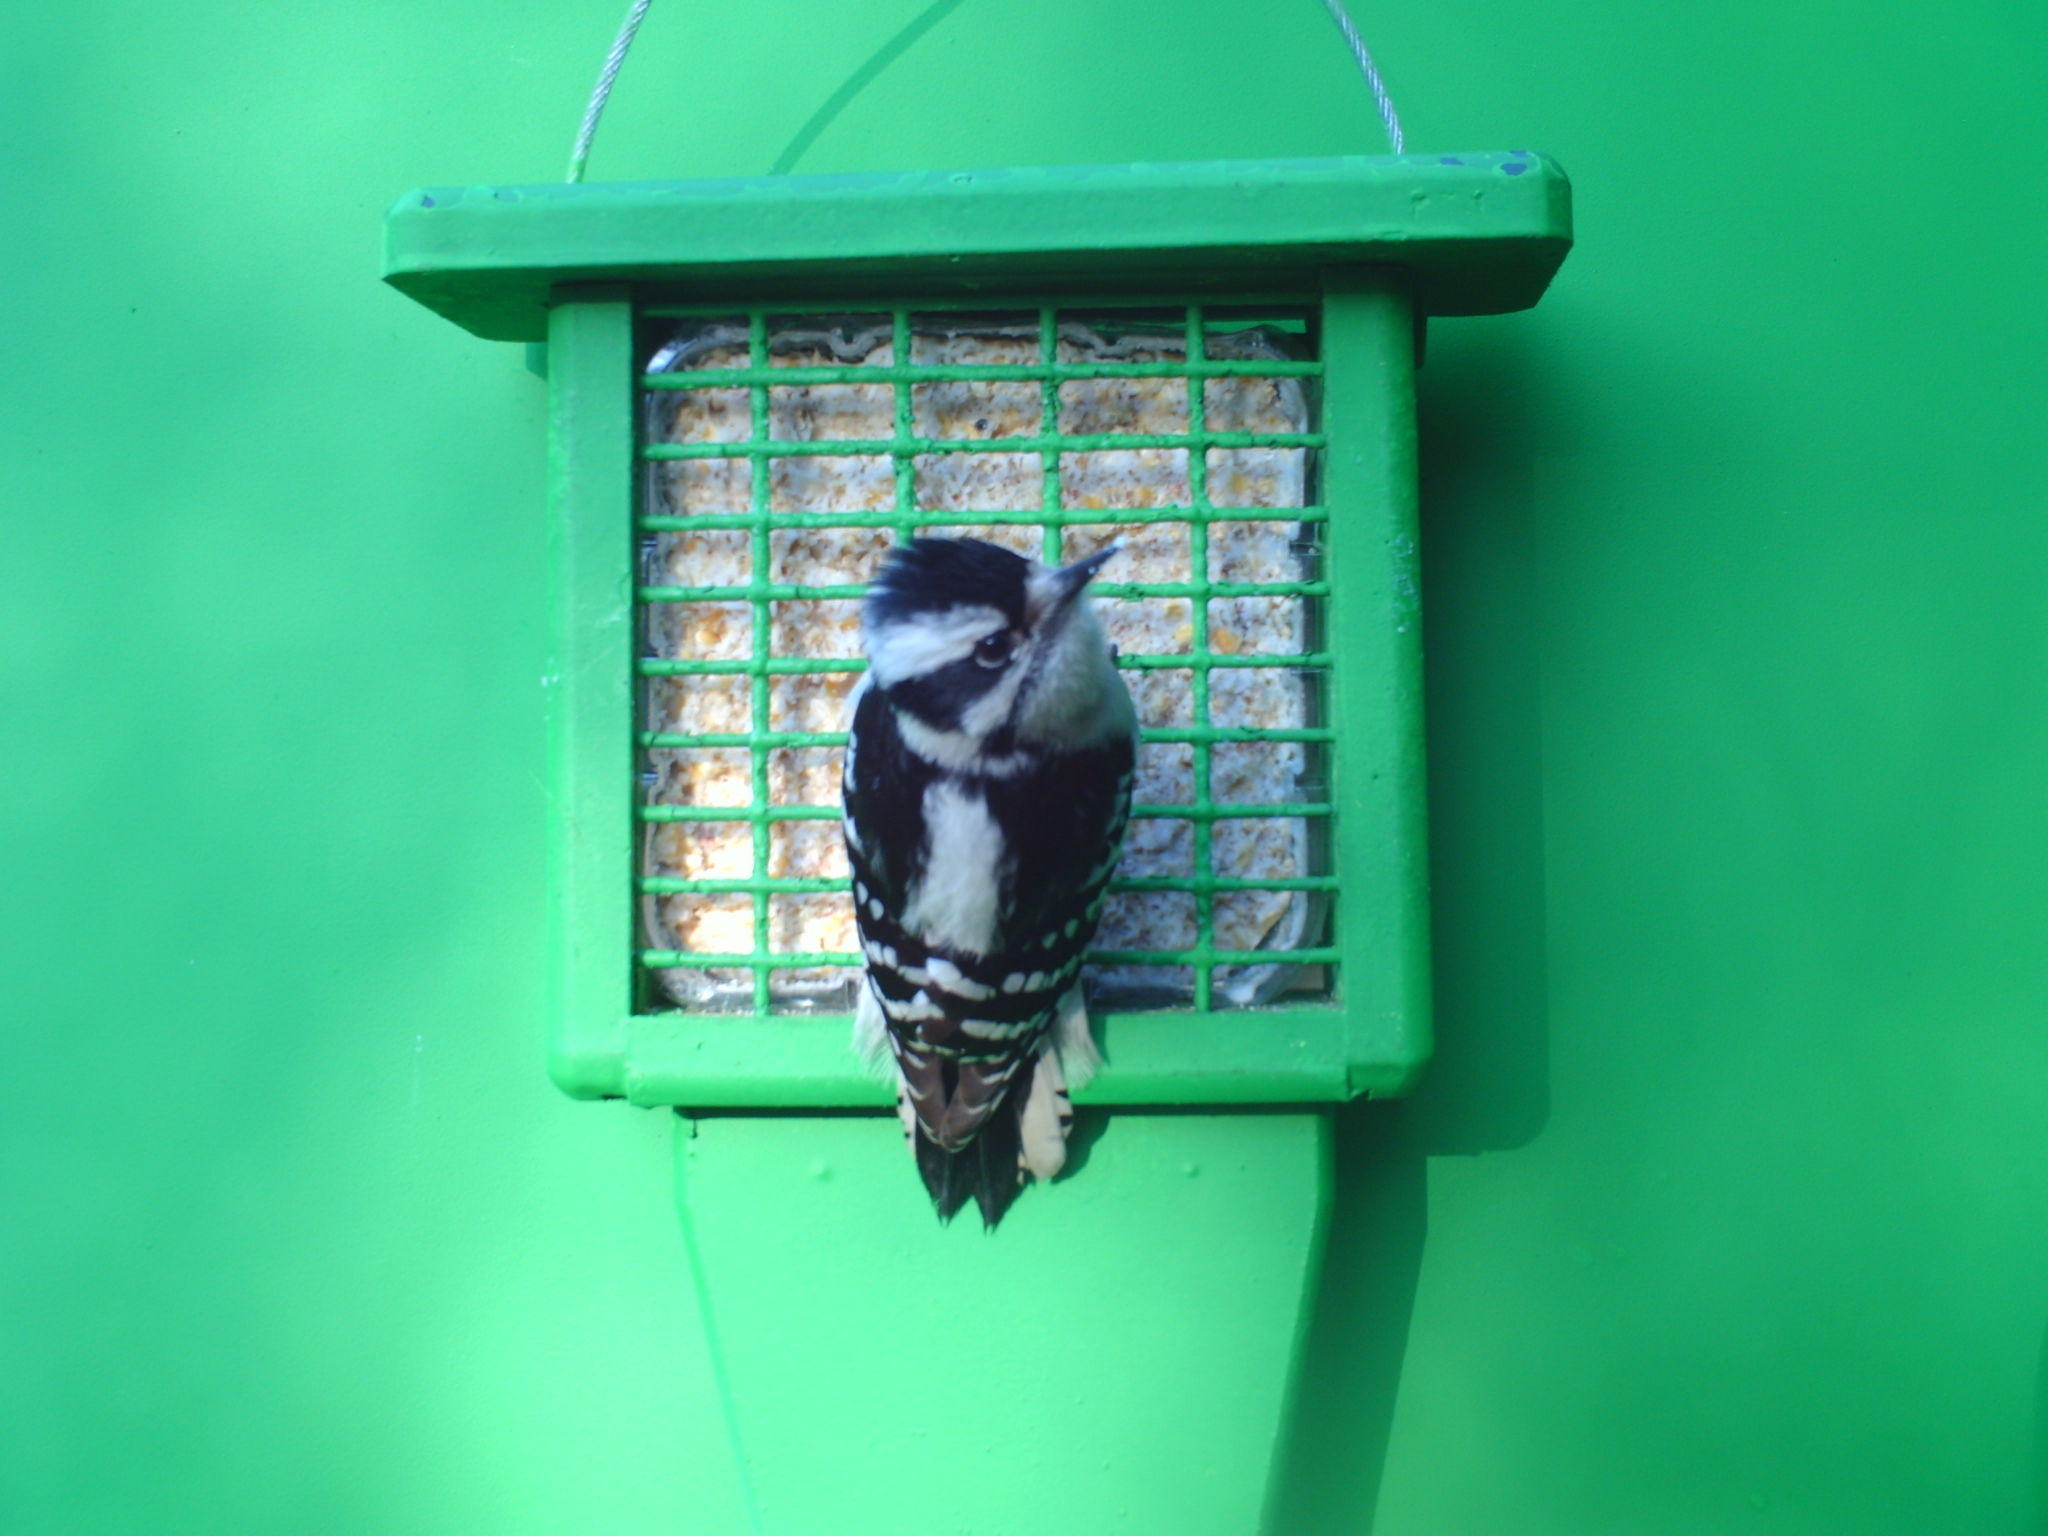
\includegraphics[width=1.5in]{images/typical.jpg}}
  \hspace*{1em}
  \subfloat[Hard shadows]{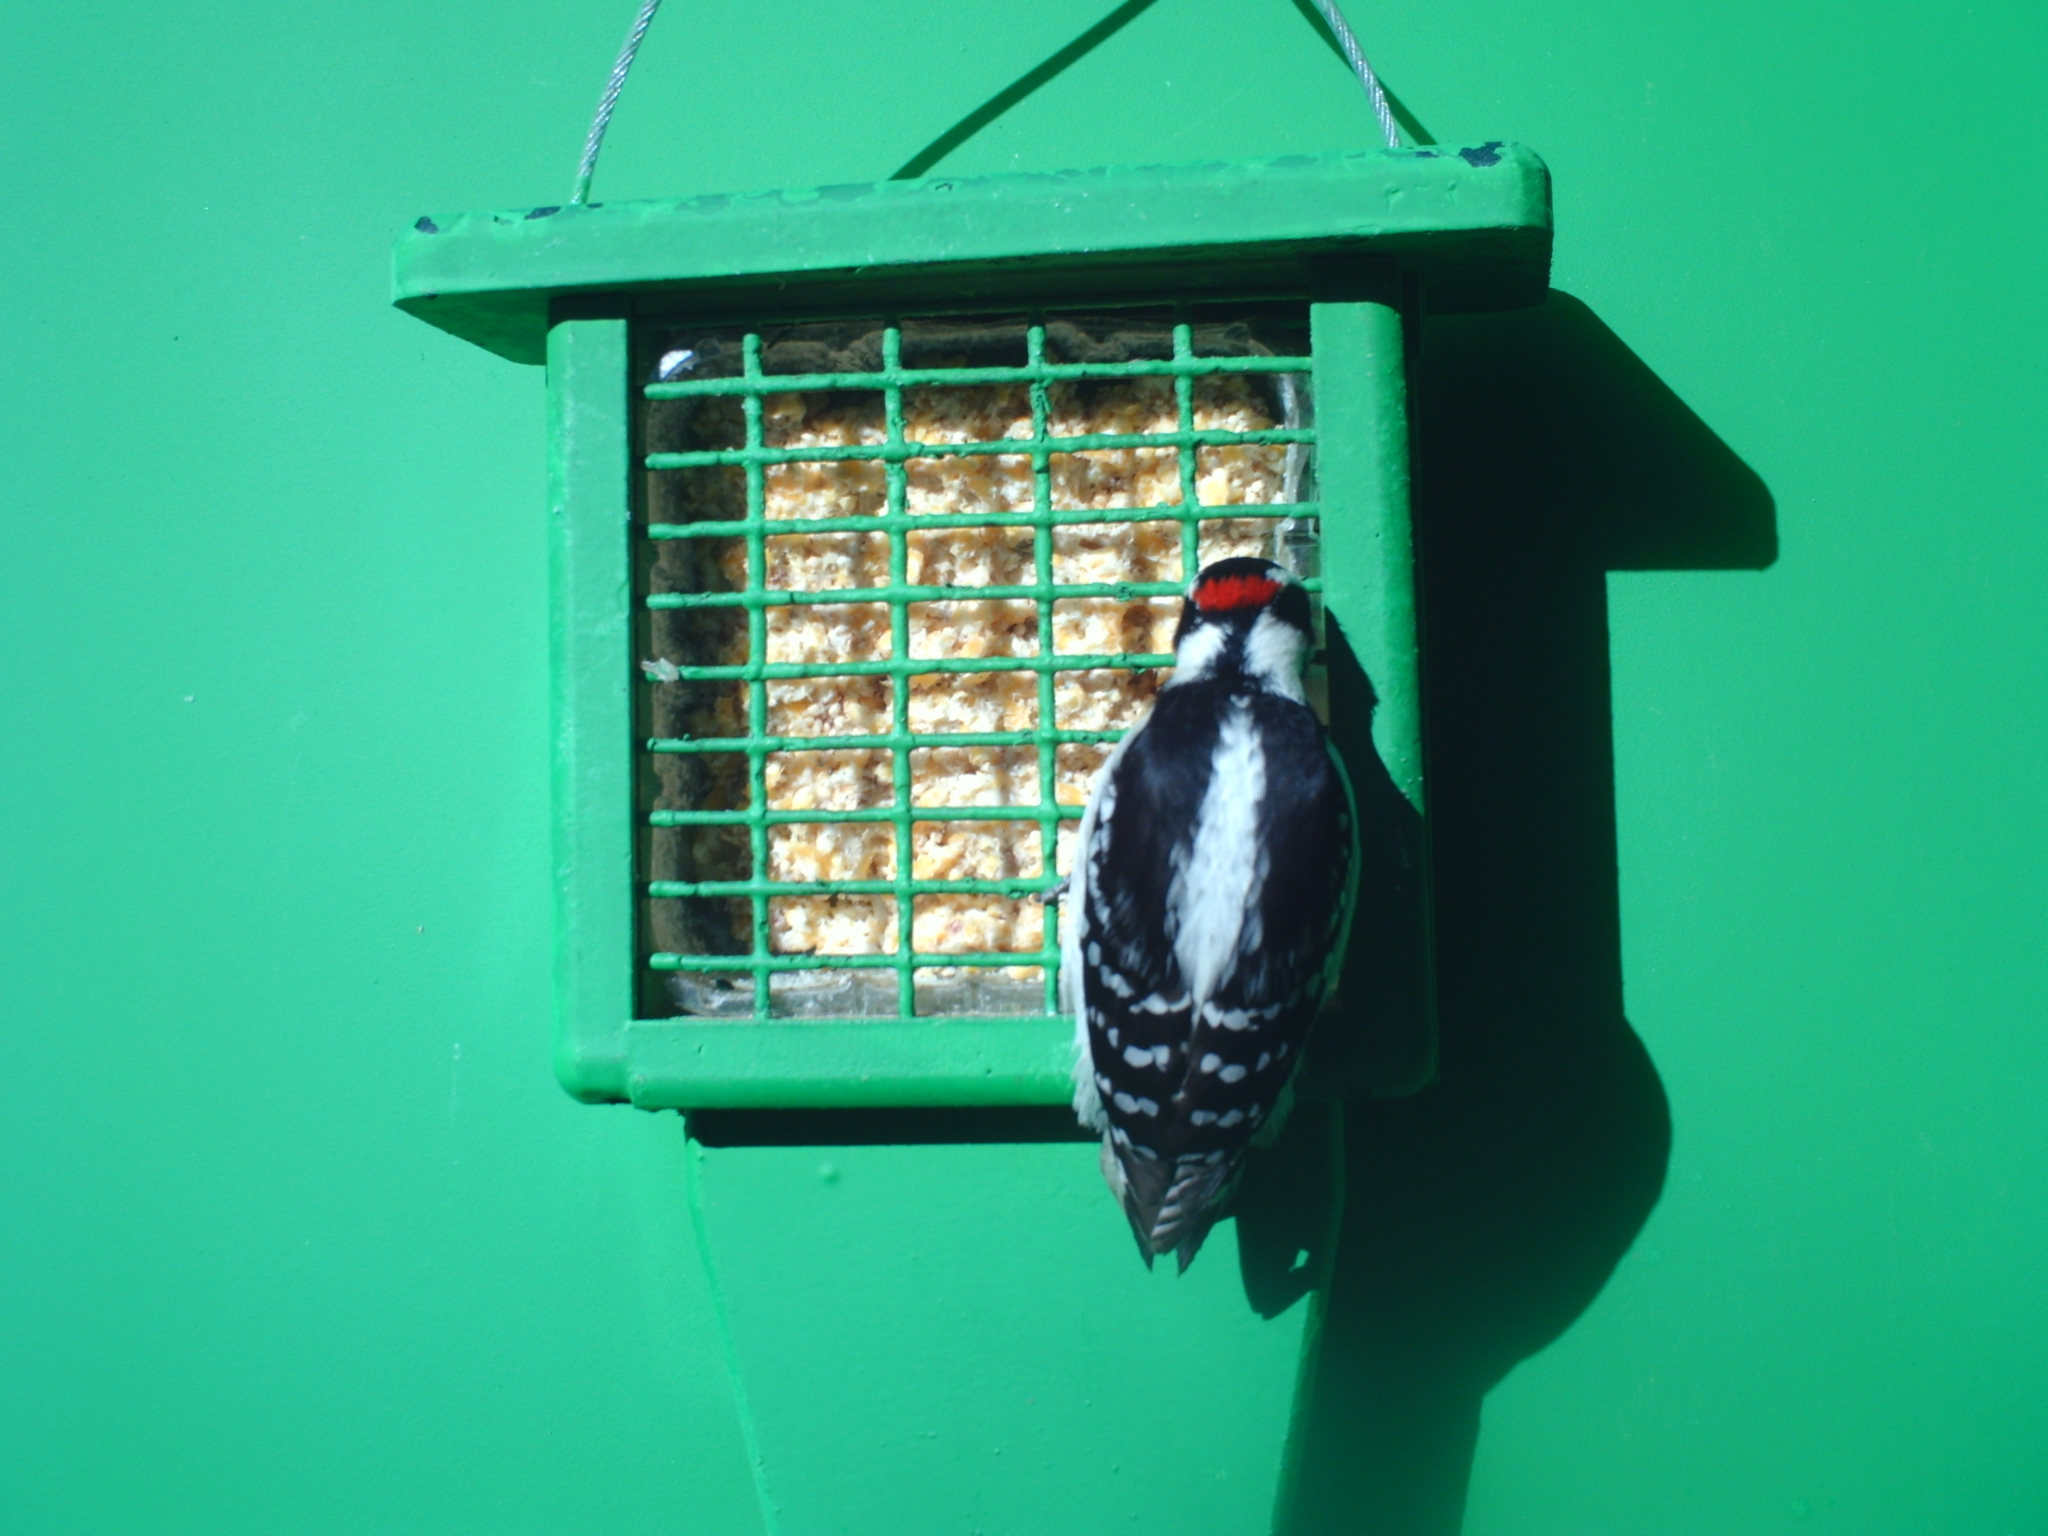
\includegraphics[width=1.5in]{images/bright.jpg}}
  \caption{Some typical images. \label{fig:TypicalImages}}
\end{figure}



  

\paragraph{Convolutional neural network architecture}

Describe how your CNN was set up.

\section{Results}
\label{sec:results}

Describe how things worked.

\section{Discussion}

This section usually talks about {\em why} the results came out
as they did.

\section{Conclusions}


\section{Acknowledgments}
The author gratefully acknowledges the support of
the University of Richmond Undergraduate Research Committee.

\newpage

\bibliographystyle{abbrv}
\bibliography{../birdid_bib/birdid.bib}

\end{document}
